\chapter{Work Done}\label{C:workdone}

\section{Overview}

The ability to trace java unit tests and perform several different analysis metrics has been implemented. For this to be achieved, several factors had to be completed and these are explored in this chapter. The different types of spectra are looked at in Section \ref{S:spectra}. The different types of analysis metrics are explored in Section \ref{S:metrics}. How the tracing is performed is examined in Section \ref{S:trace}, while the creation of the framework is explored in Section \ref{S:framework}. Lastly, how the benchmarks were selected is looked at in Section \ref{S:bench}.

\section{Test Spectra}
\label{S:spectra}

The idea of a spectrum was previously identified in Chapter \ref{C:intro}. A spectrum is some abstraction of the method executions during a test. This allows there to be several different types of spectra. The main three spectra examined are set, list and calling context. An example using the word kitten will be used to show them, where each letter represents a method execution.

\todo{Be explicity in TEST -> K , -> I ...}
\begin{itemize}
\item Set of method executions - where every method execution is only taken into account once (Result: 'Kiten')
\item List of method executions - where every method execution is taken into account, including duplicate calls (Result : 'Kitten')
\item Calling Context - for each method call, the data contains a separate node for each call stack that the method was called with \cite{callingcontext} (Result : 'k, k $\rightarrow$ i, i $\rightarrow$ t ...) 
\end{itemize}
These spectra will be analysed by different metrics to determine the level of redundancy between two tests. This is achieved in Java by examining the stack trace of the method call, where it gives information on the calling tree for that method execution. In the next section, two different analysis metrics are introduced and examined.

\section{Analysis Metrics}
\label{S:metrics}

The first metric is the Levenshtein distance between two tests spectra. This metric is the minimal number of operations that can be done to make one tests spectrum equal to another. These operations are inserting, deleting or substituting method calls and a cost is associated with completing an operation. The max difference is the size of the larger of the two spectra's. The amount of redundancy is calculated by dividing the cost of operations with the max difference in order to normalize the value. \todo{Explain minimization}

If we look at an example using a list spectra, where 'kitchen' is being compared to 'kitten' then we will have to do the following changes.

\todo{Put into a structured table to show more clearly. Unsure how.}
\begin{enumerate}
\item kitten $\rightarrow$ kitcen (Substitution of 't' with 'c')
\item kitcen $\rightarrow$ kitchen (Insertion of 'h' between 'c' and 'e')
\end{enumerate}

This shows the number of operations needed is 2, and the max is 7 as kitchen contains 7 characters. The redundancy is calculated by subtracting 1 from the cost over the max potential cost. So these two words contain 71\% redundant information. 

The second metric was determining the total difference between two spectra. This metric disregarded the calling order of a spectra, which is comparable to looking at the coverage as done in several papers \cite{fraser2007redundancy,koochakzadeh2009test,zhang2011empirical,jeffrey2005test}. The metric sorts the method calls of a spectra in alphabetical order and increments a value by 1 for each difference there is between two tests spectra. Resulting in the total difference between two tests. This value is then divided by the max possible value, which would occur when every method call is different becoming the length of both spectra, to produce a normalized redundancy value. This metric is also minimization.

Using the same spectra example as above, we need to rearrange 'kitchen' and 'kitten' into alphabetical order before calculating the redundancy, 'cehiknt' and 'eikntt' respectively.

\todo{Put into a structured table to show more clearly. Unsure how.}
\begin{enumerate}
\item Remove 'c' from 'cehiknt', increment value by 1
\item 'e' is contained in both, remove from both
\item Remove 'h' from 'hiknt', increment value by 1
\item 'iknt' is contained in both, remove from both
\item Remove 't' from 't', increment value by 1
\end{enumerate}

The total difference between the two is 3. While the max would be if they were both completely different which is 13. The redundancy is calculated by subtracting 1 from the cost over the max potential cost. The outcome being that the two words are 77\% redundant.

Maurer et al. \cite{koochakzadeh2009test} and Robinson et al. \cite{li2008static} found that test cases often had a set of methods that were in every test, such as setup and tear down. These common methods could create false positives. To understand why, a redundant test is one where it is nearly or exactly a replication of another test. Since each method call within an spectra has the same weighting, the more setup and teardown calls made means that the execution stage has decreased weighting overall. So the idea in weighting is to increase the 'importance' of lower frequency method calls by discarding the top 20\% method calls. This weighting will be added into a spectrum, where the spectrum will ignore the top 20\% method calls.

\section{Tracing}
\label{S:trace}

David Pearce's language Whiley is written in Java. Therefore it was decided to use Java to trace a tests spectrum. There are two viable options, the Java Debugging Interface (JDI) or AspectJ. JDI is similar to using an observer pattern. When a method is called, the listening trace class will be notified. In contrast, AspectJ utilises byte code weaving; this is when a piece of code is added to existing code without modifying the code itself. It uses a point cut to identify what code is weaved and where in the code \cite{aspectwiki}. A point cut is made in every method call, this point cut calls a static method in a tracer class, passing it the information about the method execution. AspectJ allows for several methods to achieve tracing through byte code weaving:

\begin{itemize}
\item Compile time:
The classes are compiled with the aspect weaved into them. So that when the jar is executed, the methods have the byte code from the aspect weaved into it already.
\item Load time:
This involves binary weaving deferred until the point in which a class loader will attempt to load in a class file.
\end{itemize}

Load time allowed for ease of use when working with external benchmarks as it only required AspectJ's class loader to be used instead through a command line flag of rebuilding the benchmarks with the AspectJ compiler.

In regard to JDI or AspectJ, AspectJ allows for more ability to choose which methods to record and making it easier to retrieve parameter values, JDI was faster to execute but provided less documentation. The decision to use AspectJ was based off this trade off between more information and performance. The analysis framework was able to be altered to increase the performance of it, so having the extra information that AspectJ gave was more important than an taking less time to execute.

\section{Framework}
\label{S:framework}

The spectrum of every test has to be compared to that of every other test in order to identify redundant test cases. The metrics identified become computationally heavy with thousands of test cases containing a spectrum consisting of tens of thousands of methods calls. To perform an analysis on that scale would take several days. A pipeline combined with time reduction strategies was determined to be the best solution.

A pipeline approach is shown in Figure \ref{fig:pipeline}. The analysing stages can be set by the user within a properties file, where they can select the spectra type, analysis metric to use and level of redundancy for each. This allows execution of reduction strategies before executing more computationally heavy analysis.

\begin{figure}[h] \todo{Change method to stage}
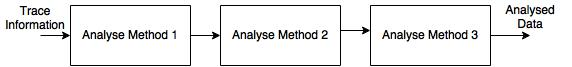
\includegraphics[width=\textwidth]{Pipeline.jpg}
\caption{Trace information goes in at the start of the pipeline. After each stage there will be a reduction of comparisons that the next stage has to complete. The last stages should be the most computationally heavy.}
\label{fig:pipeline}
\end{figure}

There were two approaches that were used to reduce the amount of analysis time. They were - implementing a heuristic and using concurrent execution. 

The heuristic looked at set of method calls, rather than a list. This meant the number of comparisons decreased. Using a 99 percent similarity for the heuristic on the wyc package of Whiley, this decreased the comparisons from stage 1 having 187922 to stage 2 with 232. 

The following illustrates an example of this.

$K,I,T,C,H,E,N \neq K,I,T,E,N,Z $

In this case, the two test cases would not be redundant due to them having a large difference in method calls.

$K,I,T,C,H,E,N \approx K,I,T,C,H,N$

There is a chance that these two may be redundant so it implies more computational heavy analysis should be done, such as analysing the list spectra. 

Concurrent execution was implemented by splitting the test cases up into 8 different parts, each part knew the test cases that it had to compare. A new thread was run to execute the comparisons, making the implementation relatively easy. The concurrent execution lead to a decrease in roughly 2 times the time taken to analyse the spectra's \todo{Maybe redo sentence}. A concurrent execution lead to an increase in memory consumption.
The analysis time had been reduced drastically, however, to run a pipeline the test suite had to be re run each time. With up to tens of thousands of tests, this could take several hours. The solution was to save the spectra data to disk.

\section{Benchmarks}
\label{S:bench}
Suitable benchmarks had to be found to test the different metrics on. They were located by looking at popular java framework's, Github repositories and David Pearce's personal projects. The benchmarks had to meet a criteria where they were Java based, had large number of test cases (100 +) and were open source. Although there were over ten potential benchmarks, the ability to use them depended on their build process. If they used Maven, it was difficult to create a jar that contained the tests and often meant that the amount of effort needed to get a working benchmark was higher than the benefit from it. This eliminated several potential benchmarks and left the Ant and gradle built projects. 

The current set of benchmarks is as follows:

\todo{Also mention the number of tests that each has and mention authors}
\textbf{Large Test Suite}
\begin{itemize}
\item Whiley
\item Spring - Core
\item Metric-x - Core
\item Ant
\end{itemize}
\textbf{Small Test Suite}
\begin{itemize}
\item Java Compiler Kit
\item Jasm
\end{itemize}
